\documentclass[11pt]{article}

\usepackage[a4paper,margin=2.5cm]{geometry}
\usepackage{graphicx}
\usepackage{tabularx}
\usepackage{booktabs}
\usepackage{hyperref}
\usepackage{xcolor}
\usepackage{enumitem}
\usepackage{parskip}

\graphicspath{{figures/}}

\hypersetup{
  colorlinks=true,
  linkcolor=blue,
  urlcolor=blue,
  citecolor=blue,
}

\title{Autonomous Driving Project --- Documentation}
\author{TUM ``Introduction to ROS'' 2026 --- Autonomous Driving group project}
\date{}

\begin{document}
\maketitle

This document explains the architecture, design decisions, external
dependencies, known limitations, and results of our submission. See the
repository \texttt{README.md} for install/build/run instructions.

\section{System Overview}

The car drives a fixed \textasciitilde{}785\,m urban loop published once at
startup from a pre-recorded, lane-snapped set of waypoints. Five ROS~2
packages we wrote ourselves sit on top of two packages provided by the
course (\texttt{simulation}, the Unity TCP/UDP bridge, and
\texttt{dummy\_controller}, an unused reference example) and several
external ROS libraries:

\begin{verbatim}
Unity sim  <--TCP/UDP-->  simulation (course-provided bridge)
                                |
                                v
                    depth image, RGB image, pose, twist
                                |
        +-----------------------+------------------------+
        v                                                 v
   perception                                          planning
   (obstacle_guard_node,                          (route_planner_node:
    traffic_light_node,                            waypoints -> speed
    + octomap_server for a                          profile -> trajectory,
    supplementary curb check)                        detour replanning)
        |                                                 |
        +-----------------------+------------------------+
                                v
                            control
                    (pure_pursuit_node: path
                     tracking, ACC, traffic-light
                     state machine, detour/verify
                     state machine, emergency stop)
                                |
                                v
                       /car_command -> simulation -> Unity
\end{verbatim}

A single launch file (\texttt{bringup/main.launch.py}) starts every node,
the static TF tree, and RViz. See Section~\ref{sec:rosgraph} for the full
ROS graph.

\section{Packages and Nodes}

\begin{table}[h]
\small
\begin{tabularx}{\textwidth}{@{}l l l X@{}}
\toprule
\textbf{Package} & \textbf{Owner (EDIT)} & \textbf{Node(s)} & \textbf{Responsibility} \\
\midrule
\texttt{simulation} & \emph{course-provided} & \texttt{unity\_TCP\_stream\_receiver}, \texttt{ROS\_command\_transmitter} & TCP/UDP bridge to Unity: publishes ground-truth pose/twist, RGB/depth/semantic camera, IMU; sends \texttt{VehicleControl} commands. Ported to ROS~2 Jazzy from the course's original package, not otherwise modified. \\
\texttt{dummy\_controller} & \emph{course-provided} & --- & Minimal example controller from the course. Not used by \texttt{bringup}; kept only for reference. \\
\texttt{project\_interfaces} & Author 1 & --- & Our custom message types: \texttt{Trajectory}/\texttt{TrajectoryPoint} (planned path with per-point speed) and \texttt{TrafficLight} (detected signal state). \\
\texttt{perception} & Author 2 & \texttt{obstacle\_guard\_node} & Transforms the depth-camera point cloud into the world frame and measures, along the upcoming planned trajectory, the arc-length distance to the nearest obstacle in four corridors (main/tight/overtake-left/overtake-right), plus a supplementary check against an accumulated OctoMap projection for low obstacles (curbs) the live per-frame scan can't see (Section~\ref{sec:control}). \\
\texttt{perception} & Author 2 & \texttt{traffic\_light\_node} & RGB HSV blob detection of the facing signal head. Deliberately does \textbf{not} use the semantic camera (bonus criterion). \\
\texttt{planning} & Author 3 & \texttt{route\_planner\_node} & Builds a lane-snapped, curvature-limited-speed trajectory from the recorded waypoints; reactively replans a lateral detour around a confirmed static obstacle; selects the nearest still-ahead goal from the task's predefined pose list. \\
\texttt{control} & Author 1 & \texttt{pure\_pursuit\_node} & Pure-pursuit path tracking, ACC-style gap control, traffic-light stop/go state machine, detour engage/verify/thread/hold state machine, emergency braking. Implements the required \texttt{/control/enable} service. \\
\texttt{bringup} & Author 3 & --- & Single launch file, static TF tree (sensor extrinsics per the task sheet's vehicle drawing), RViz config. \\
\bottomrule
\end{tabularx}
\end{table}

\subsection{Perception}

\texttt{obstacle\_guard\_node} receives the depth camera's point cloud
(converted to \texttt{sensor\_msgs/PointCloud2} by the external
\texttt{depth\_image\_proc} component), transforms every point into the
world frame via \texttt{tf2}, and classifies each against the closest
segment of the currently-planned trajectory. Points with world height in
$[0.35, 3.0]$~m are kept (below that is road-surface noise and low
sidewalk fringes); four corridor distances are published, including a
\texttt{tight} corridor used both for ACC following and for verifying a
detour path is actually clear before committing to it.

\texttt{traffic\_light\_node} classifies connected components in an
HSV-thresholded mask of the facing camera image, filtering blobs by shape
(compact, roughly square, well-filled) to reject false positives such as
the red ring of no-U-turn signs or red shop banners. Only red and green
are detected --- the amber phase is skipped because the signal casing is
itself amber-painted metal and cannot be reliably separated from a lit
amber lamp; the controller treats ``stopped, no fresh green yet'' as
``keep waiting,'' which is compliant behaviour.

\subsection{Planning}

\texttt{route\_planner\_node} loads the recorded waypoints, builds a
curvature-limited speed profile, and publishes a \texttt{Trajectory}. On a
\texttt{/planning/detour} request from \texttt{control} it re-splices a
laterally-offset segment around a confirmed static obstacle, then restores
the base route once past it. It also implements short-term goal selection
over the task's predefined pose list (Fig.~4 in the task sheet): each pose
is projected onto the route's arc length once at startup, and the nearest
goal still ahead of the car is published (on change only) to
\texttt{/planning/current\_goal}.

\subsection{Control}
\label{sec:control}

\texttt{pure\_pursuit\_node} tracks the published trajectory with a
standard pure-pursuit lateral law and a throttle law combining a
feed-forward table (calibrated against the simulator's own speed-tracking
deficit) with proportional correction. On top of that:

\begin{itemize}[leftmargin=*]
\item \textbf{ACC-style gap control} slows for anything in the
  tight/main corridor ahead, with a distance-scaled approach cap.
\item \textbf{Traffic-light state machine} stops at the correct stop line
  for a red phase and releases on a confirmed green; a bounded
  blind-release timer covers the one junction (TL4) whose signal head
  leaves the camera's field of view right at the stop line --- see
  Section~\ref{sec:limitations} for the honest limitation here.
\item \textbf{Obstacle detour state machine}
  (\texttt{kNormal -> kVerify -> kDetour}, with a \texttt{kHold} fallback)
  proactively replans around a static obstacle once confirmed parked
  (tracked as static vs.\ moving by watching its world position over a
  few seconds), verifies the shifted path is clear before committing, and
  threads it.
\item \textbf{Emergency stop}: every control tick, independent of the
  above, computes the deceleration required to stop before the nearest
  raw corridor obstacle ($a = v^2 / (2d)$) and immediately commands full
  brake if that exceeds a threshold --- this is the task's Event~II
  (``NPC crosses then brakes hard'') handling.
\item \textbf{Supplementary OctoMap cross-check}: \texttt{obstacle\_guard\_node}
  also publishes \texttt{/perception/map\_tight\_distance}, sourced from
  \texttt{octomap\_server}'s accumulated occupancy map (height-banded to
  0.08--0.35~m, exactly the range the live per-frame corridor filter
  ignores) rather than the instantaneous point cloud. \texttt{kVerify}
  ANDs this into its detour-clear check: a fresh map hit can additionally
  veto a detour the live sensor alone would have approved (catching a
  curb the live sensor structurally cannot see), but a stale or absent
  reading never blocks anything by itself. Two bounded-trust safeguards
  keep this from ever causing an indefinite hold: the map signal is
  judged stale (and ignored) if the underlying map itself hasn't been
  updated recently, and a map-only block (live sensor says clear) can
  hold for at most 25~s before the system falls back to trusting the
  live sensor alone.
\end{itemize}

\section{ROS Graph}
\label{sec:rosgraph}

\begin{figure}[h]
  \centering
  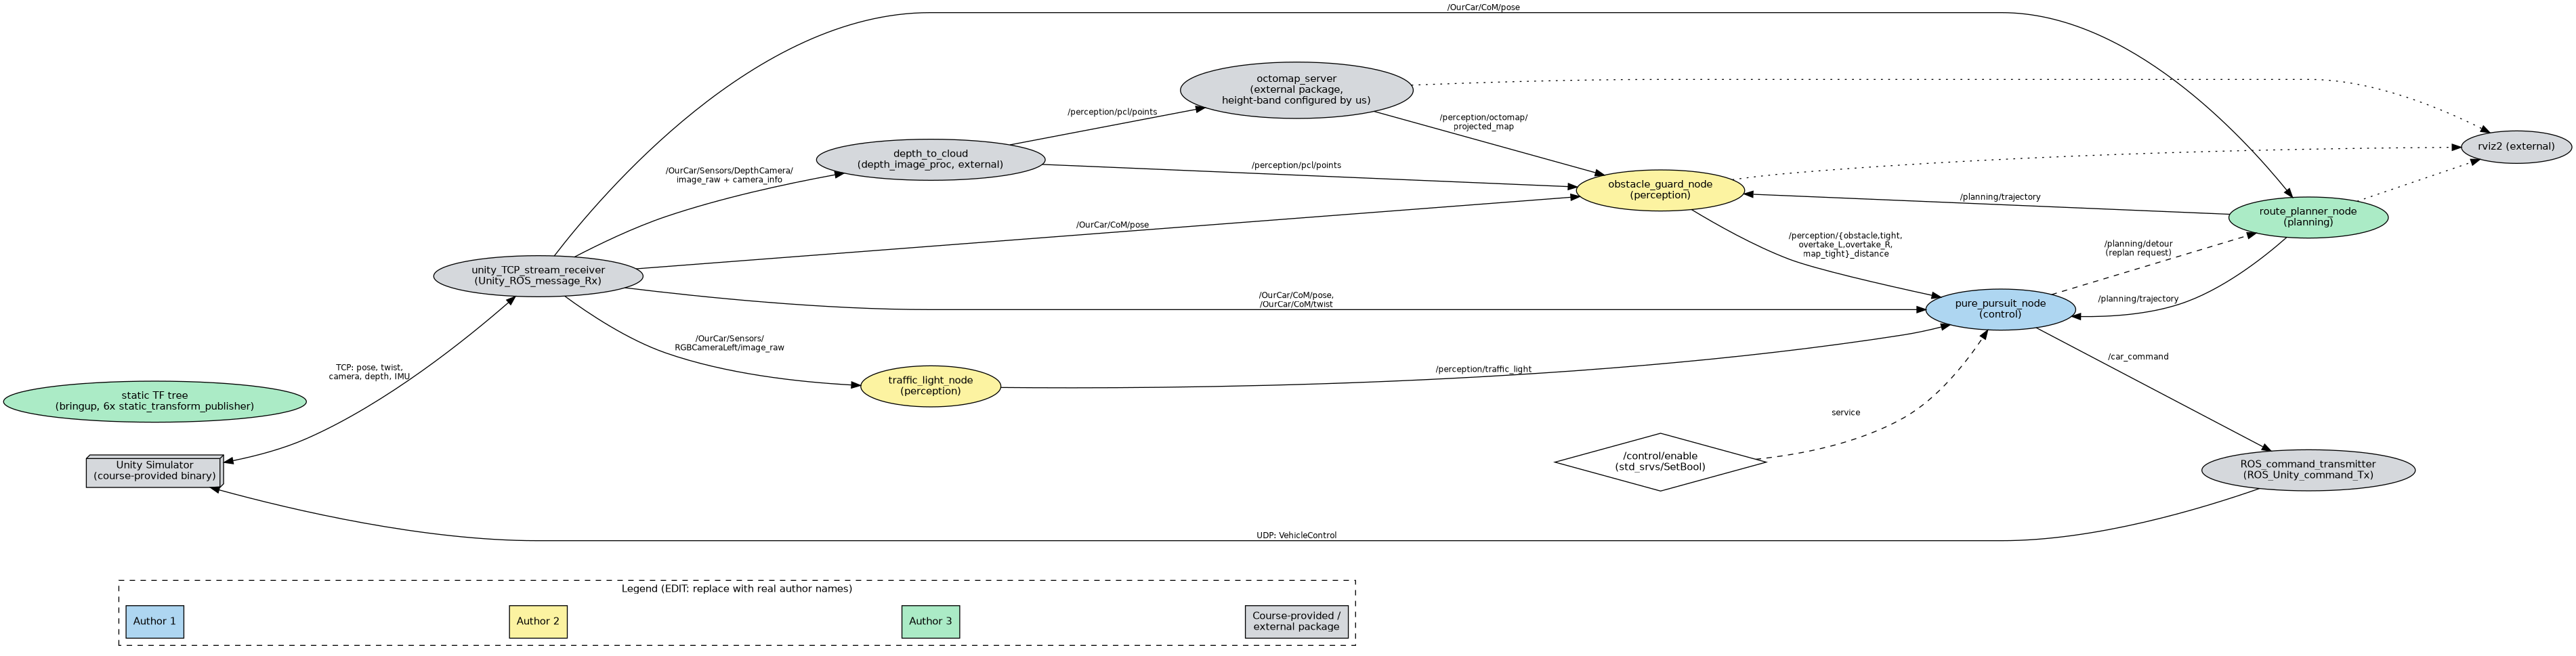
\includegraphics[width=\textwidth]{ros_graph.png}
  \caption{ROS computation graph, colored by author. Author colors are
  placeholders --- see the table in Section~2 for the current mapping;
  replace with real names before submission.}
\end{figure}

\section{Results}

A full, uninstrumented run of the finished system
(\texttt{bringup/main.launch.py}, default parameters): \textbf{272\,s,
zero collisions, zero stalls, one detour, two red-light stops handled
correctly}, matching the same events/timing observed across every
regression run in this development cycle (the detour always engages at
the same static obstacle, both traffic lights always transition
red$\to$green cleanly with no flicker).

\begin{itemize}[leftmargin=*]
\item Average speed \textbf{2.7\,m/s}, peak \textbf{7.5\,m/s} on the two
  longest clear straights.
\item Figure~\ref{fig:speedmap} shows the driven path colored by
  instantaneous speed --- the dark (near-zero) points mark the detour and
  the two traffic-light stops; speed climbs highest on the long straights
  on either side of the loop.
\item Figure~\ref{fig:speedprofile} shows the same data as speed vs.\
  distance travelled: five visible near-zero dips (the detour's
  approach-and-verify wait plus a couple of ACC-queueing slowdowns, and
  the two full traffic-light stops), with the car re-accelerating
  smoothly after each.
\item The distance-travelled axis reads \textbf{\textasciitilde{}721\,m}
  rather than the route's documented \textasciitilde{}785\,m: it's a
  straight-line, point-to-point Euclidean sum over 10\,Hz pose samples,
  which undercounts on curves (chord vs.\ arc) --- a measurement-method
  artifact, not a shorter drive.
\item Figures~\ref{fig:routemap} and \ref{fig:tracktraced} show the
  planned route overlaid on the course map, generated during
  route-planning development.
\end{itemize}

\begin{figure}[h]
  \centering
  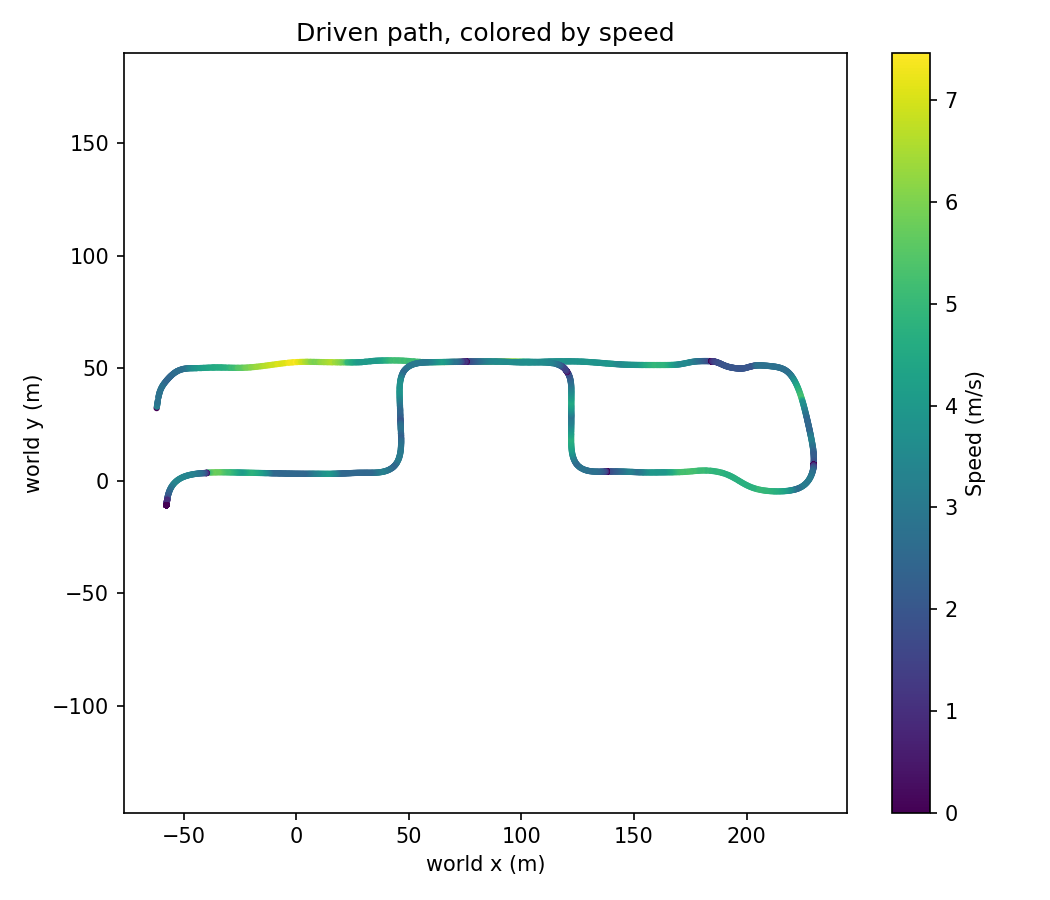
\includegraphics[width=0.75\textwidth]{route_speed_map.png}
  \caption{Driven path, colored by instantaneous speed.}
  \label{fig:speedmap}
\end{figure}

\begin{figure}[h]
  \centering
  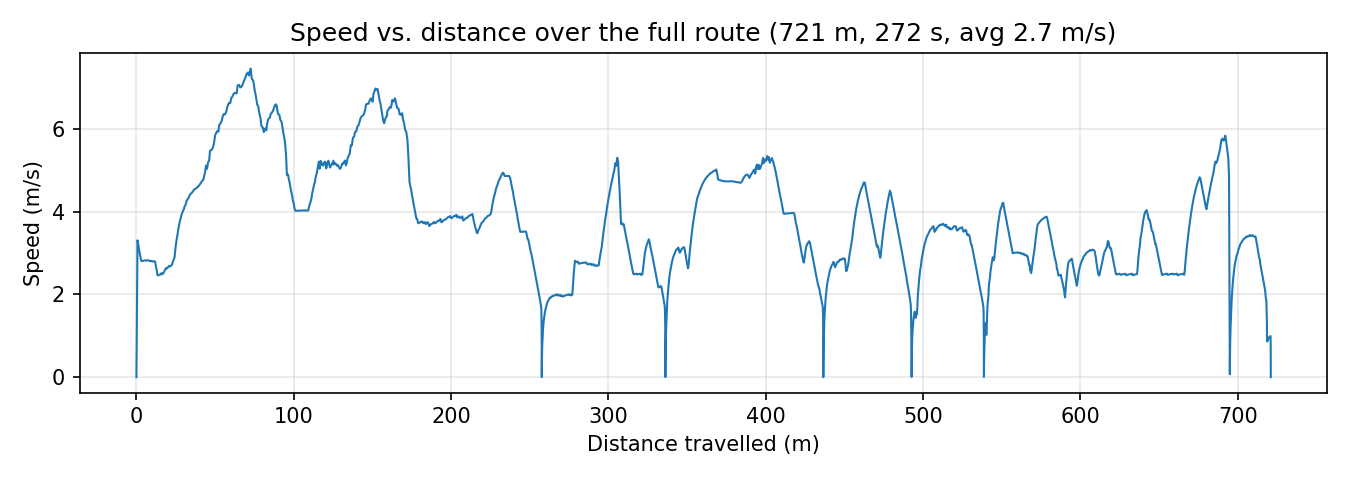
\includegraphics[width=\textwidth]{speed_profile.png}
  \caption{Speed vs.\ distance travelled over the full route.}
  \label{fig:speedprofile}
\end{figure}

\begin{figure}[h]
  \centering
  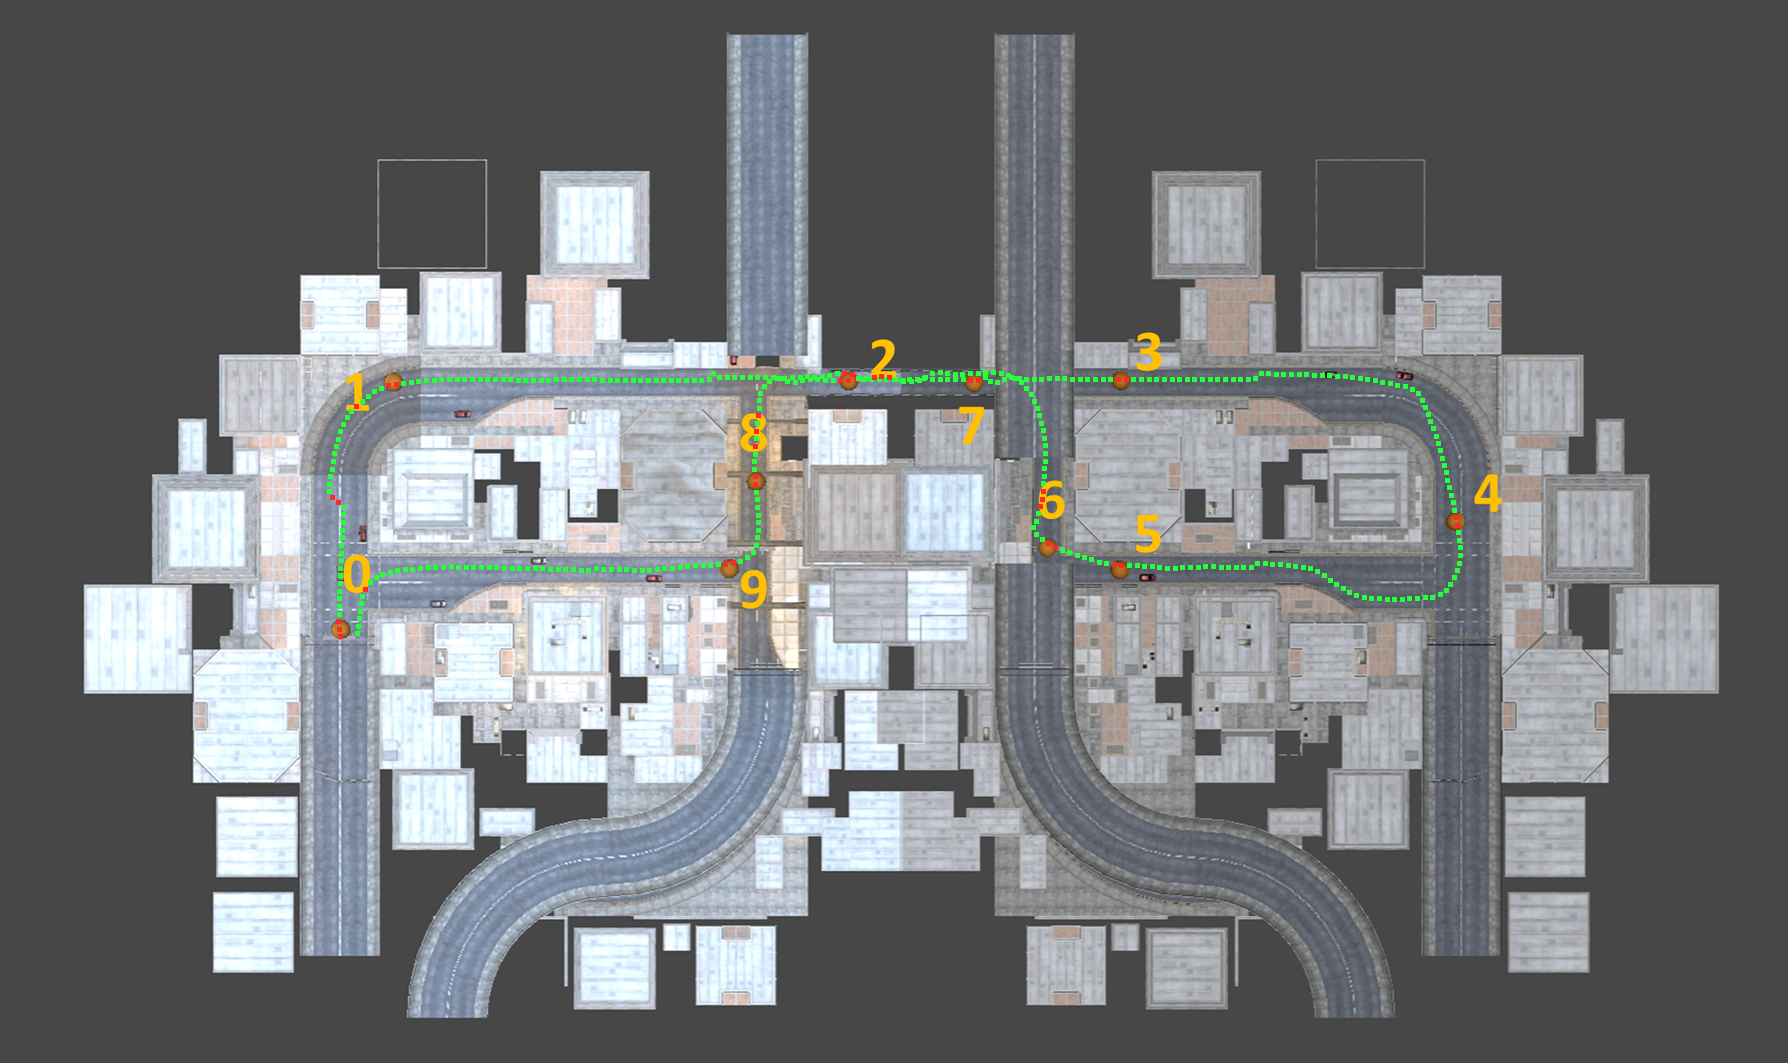
\includegraphics[width=0.75\textwidth]{route_on_map.png}
  \caption{Planned route overlaid on the course map.}
  \label{fig:routemap}
\end{figure}

\begin{figure}[h]
  \centering
  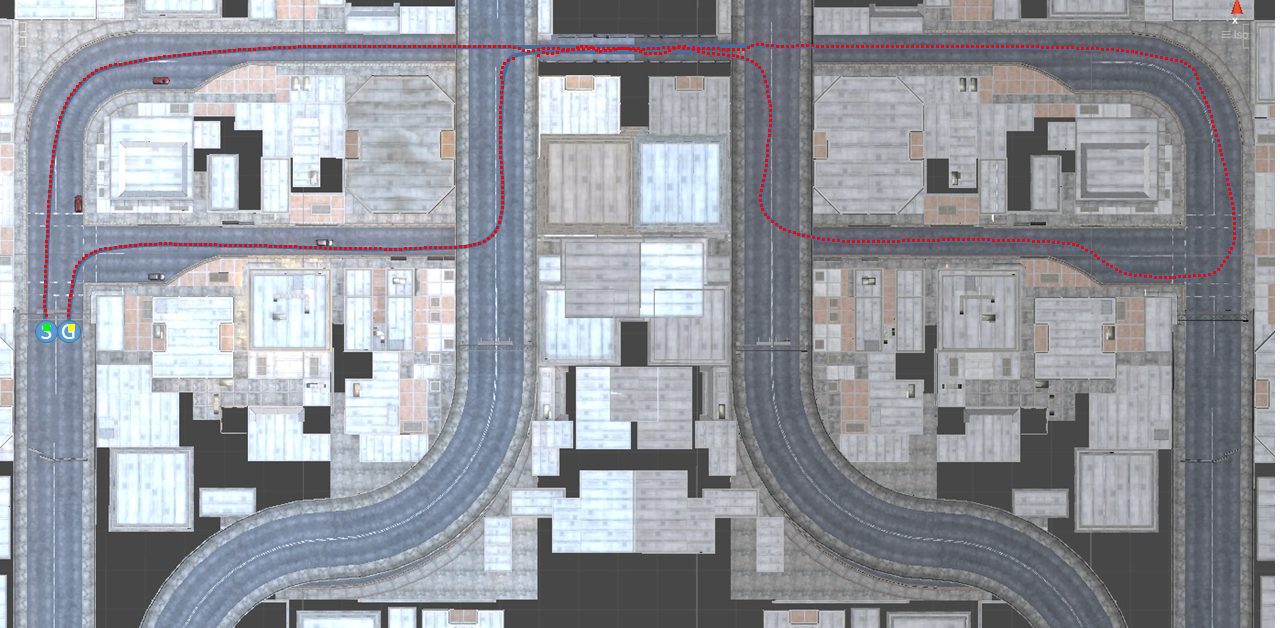
\includegraphics[width=0.75\textwidth]{track_traced.png}
  \caption{Traced track used for waypoint generation.}
  \label{fig:tracktraced}
\end{figure}

\section{Known Limitations / Requirements Not Fully Met}
\label{sec:limitations}

\begin{itemize}[leftmargin=*]
\item \textbf{TL4 blind-release timing}: this junction's signal head
  becomes detectable only right at the stop line, so the car sometimes
  has to release from the stop without a confirmed-fresh phase reading.
  The release timer is bounded by the junction's own measured red-phase
  duration, but the red phase (22\,s) is longer than the following
  green+amber window (14\,s) --- for \emph{any} fixed-delay timer with no
  live visibility, there exists an arrival phase-offset where release
  lands inside the \emph{next} red phase (worst case \textasciitilde{}8\,s
  of unavoidable overlap). We removed one avoidable failure mode (a late
  transient vote extending the wait past the intended point) but this
  residual risk is a physical limitation of the intersection's geometry
  versus its light timing, not something a control-side fix alone can
  eliminate.
\item \textbf{OctoMap curb cross-check} (Section~\ref{sec:control}) is
  code-reviewed and bounded-safe (verified not to introduce false blocks
  or hangs across multiple full-route regression runs) but never actually
  triggered during testing --- this route's one static obstacle doesn't
  happen to sit at curb height the live sensor misses. It is included as
  a genuine safety net for cases the live corridor structurally can't
  see, not because we observed it catching something in our own test
  runs.
\item \textbf{Perception update rate} (\textasciitilde{}0.7--1\,Hz for
  the point-cloud-derived corridor distances) is limited by the Unity
  simulator's own single-core render/physics loop, confirmed by measuring
  the same corridor rate across several different look-ahead/decimation
  settings in our own code --- not something fixable from the ROS side.
  This bounds how much cruise speed can be raised before stale-corridor
  braking becomes frequent.
\end{itemize}

\section{External Code / Not Written by Us}

\begin{itemize}[leftmargin=*]
\item \texttt{simulation}, \texttt{dummy\_controller}: provided by the
  course (maintainers Markus Ryll, Jiaming Zhang), ported to ROS~2
  Jazzy; not modified beyond what porting required.
\item \texttt{depth\_image\_proc} (\texttt{PointCloudXyzNode}),
  \texttt{octomap\_server}, \texttt{tf2\_ros}, \texttt{rviz2},
  \texttt{rclcpp}/\texttt{rclcpp\_components}, \texttt{std\_srvs},
  \texttt{cv\_bridge}, OpenCV: standard ROS~2 / third-party libraries,
  used as-is via their public APIs and launch-file parameters (not
  modified); see bibliography.
\item Everything in \texttt{project\_interfaces}, \texttt{perception},
  \texttt{planning}, \texttt{control}, and \texttt{bringup}'s launch file
  / TF tree is written by us.
\end{itemize}

\section{Team \& Contributions}

\emph{(Placeholder --- replace with real names.)}

\begin{table}[h]
\small
\begin{tabularx}{\textwidth}{@{}l X@{}}
\toprule
\textbf{Author} & \textbf{Main contributions} \\
\midrule
Author 1 & \texttt{control} (\texttt{pure\_pursuit\_node}): path tracking, ACC, traffic-light and detour state machines, emergency stop, \texttt{/control/enable} service; \texttt{project\_interfaces} message design \\
Author 2 & \texttt{perception} (\texttt{obstacle\_guard\_node}, \texttt{traffic\_light\_node}): corridor obstacle monitoring, OctoMap cross-check, HSV traffic-light detection \\
Author 3 & \texttt{planning} (\texttt{route\_planner\_node}): trajectory generation, detour replanning, goal selection; \texttt{bringup} (launch file, TF tree, RViz config) \\
\bottomrule
\end{tabularx}
\end{table}

\begin{thebibliography}{11}

\bibitem{ros2docs} Open Robotics, \emph{ROS~2 Documentation --- Jazzy Jalisco}, \url{https://docs.ros.org/en/jazzy/}, accessed 2026.

\bibitem{coulter1992} R.~C. Coulter, ``Implementation of the Pure Pursuit Path Tracking Algorithm,'' Carnegie Mellon University Robotics Institute, Tech. Rep. CMU-RI-TR-92-01, 1992.

\bibitem{hornung2013} A.~Hornung, K.~M. Wurm, M.~Bennewitz, C.~Stachniss, and W.~Burgard, ``OctoMap: An Efficient Probabilistic 3D Mapping Framework Based on Octrees,'' \emph{Autonomous Robots}, 34(3), pp.~189--206, 2013.

\bibitem{octomapserver} \texttt{octomap\_server} / \texttt{octomap\_mapping}, OctoMap project, \url{https://github.com/OctoMap/octomap_mapping}.

\bibitem{depthimageproc} \texttt{image\_pipeline} / \texttt{depth\_image\_proc}, ROS Perception, \url{https://github.com/ros-perception/image_pipeline}.

\bibitem{pcl2011} R.~B. Rusu and S.~Cousins, ``3D is Here: Point Cloud Library (PCL),'' \emph{IEEE International Conference on Robotics and Automation (ICRA)}, 2011.

\bibitem{opencv2000} G.~Bradski, ``The OpenCV Library,'' \emph{Dr. Dobb's Journal of Software Tools}, 2000.

\bibitem{tf2013} T.~Foote, ``tf: The Transform Library,'' \emph{IEEE International Conference on Technologies for Practical Robot Applications (TePRA)}, 2013.

\bibitem{rviz} Open Robotics, \emph{RViz Documentation}, \url{https://github.com/ros-visualization/rviz}.

\bibitem{unity} Unity Technologies, \emph{Unity Engine} (course-provided simulation binary).

\bibitem{tasksheet} TUM Chair of Autonomous Aerial Systems, \emph{Introduction to ROS 2026 --- Autonomous Driving Project} (task sheet), 2026.

\end{thebibliography}

\end{document}
